\documentclass[titlepage]{report}

\usepackage{setspace}

\usepackage[utf8]{inputenc}
\usepackage{amsmath}   
\usepackage{mathtools}
\usepackage{graphicx}
\usepackage{subcaption}
\usepackage{float}
\usepackage{hyperref}
\usepackage{listings}
\usepackage[labelfont=bf]{caption}
\usepackage[margin=3.5cm]{geometry}

\lstset{
	basicstyle=\footnotesize\ttfamily,
}

\title{
\vspace{60pt}\\
\huge \bfseries SKEDGE
\\
\vspace{10pt}
\Large
Smarter course scheduling for our\\
University of Rochester
}

\author{
	Dan Hassin\\
    \vspace{5pt}\\
    Supervised by\\
    Professor Philip Guo\\
    \vspace{2pt}\\
    Department of Computer Science\\
    University of Rochester\\
    Rochester, New York\\
}

\date{April 12, 2016\\
    \vspace{150pt}\\
    submitted in partial fulfillment of\\
    the requirements for the degree\\
    \emph{honors bachelor of science}\\
}

\begin{document}

\maketitle

%%%%%%%%%%%

\onehalfspacing

\pagenumbering{gobble}
\setcounter{tocdepth}{1}
\tableofcontents

\listoftables

\listoffigures

\clearpage

%%%%%%%%%%%%%%%%%%

\doublespacing

\addcontentsline{toc}{chapter}{Abstract}

\begin{abstract}

\thispagestyle{plain}
\pagenumbering{roman}

In this paper I present Skedge, a web application for students to comfortably and effectively engage with the University's course catalog. Skedge matches and surpasses the capabilities of the existing University tool for this purpose, ``Course Description / Course Schedule'' (CDCS) and presents its information in a more visually pleasing way. As a result, Skedge boasts strong user-retention rates, long session durations, and high student adoption despite having virtually no advertisement. Through collected usage data, I demonstrate that a) Skedge's differences from and additions to CDCS are usable and have real need, b) the two major use-cases associated with course browsing---direct search and exploratory search---are effectively accommodated by Skedge, and c) Skedge's search mechanism is user-friendly and self-teaches to users over time.

\end{abstract}


%%%%%%%%%%%%%%%

\pagenumbering{arabic}



\chapter{Introduction}

This paper will begin by 

\section{Overview of CDCS}

CDCS is the University's official tool for 

\label{fig:cdcs-index}

\subsection{``Better CDCS''}

%%%

\section{Overview of Skedge}

Skedge is a website I developed in 2014 and have been maintaining and developing since.

Bookmarks

Students, parents, department coordinators, and faculty can all benefit from such tool improvements.

user accounts are lightweight, no login, cookie (browser) based

\ref{fig:sk-index}


\begin{figure}[ht]
    \centering
        \begin{subfigure}[h]{14cm}
            \centering
            \fbox{
                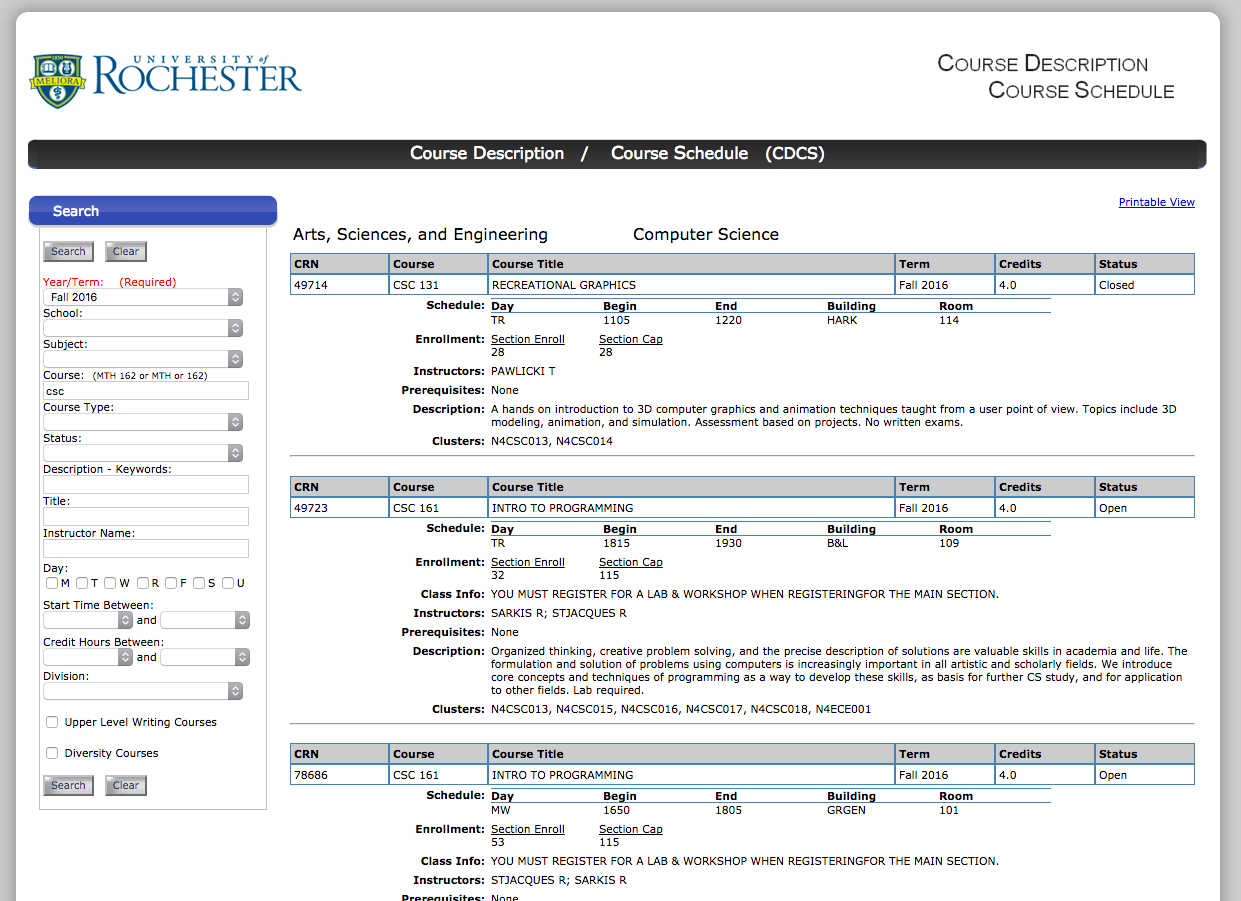
\includegraphics[width=1.00\textwidth]{images/cdcs/index}
            }
            \caption{CDCS, with the search query {\tt csc}}
            \label{fig:cdcs-index}
        \end{subfigure}\\
        \vspace{10pt}\\
        \begin{subfigure}[h]{14cm}
            \centering
            \fbox{
                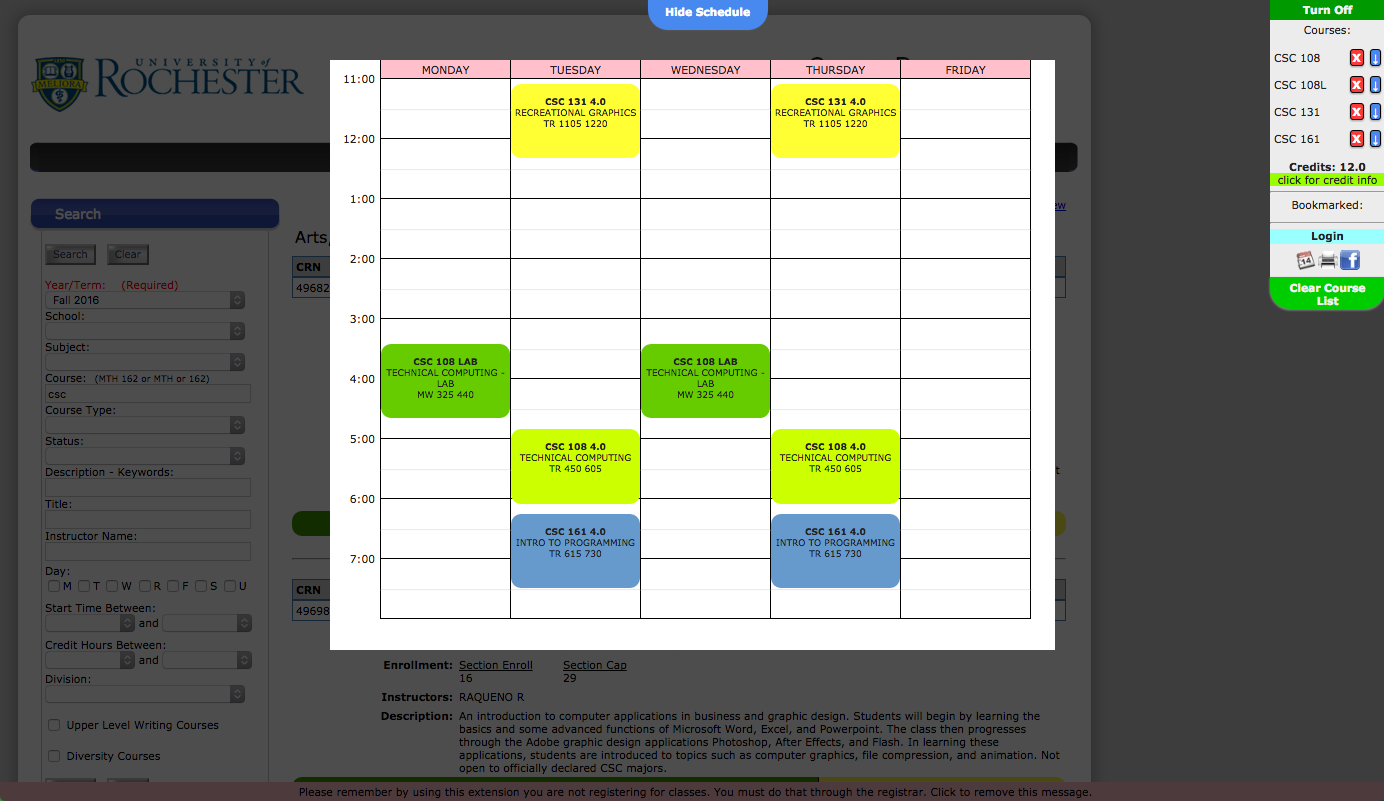
\includegraphics[width=1.00\textwidth]{images/cdcs/better}
            }
            \caption{Better CDCS, a separate browser extension that embeds buttons into the CDCS course results interface, allowing users to add courses to a locally-stored schedule}
            \label{fig:cdcs-better}
        \end{subfigure}
    \caption{CDCS and Better CDCS in their current states}
\end{figure}

\begin{figure}[ht]
    \centering
    \fbox{
        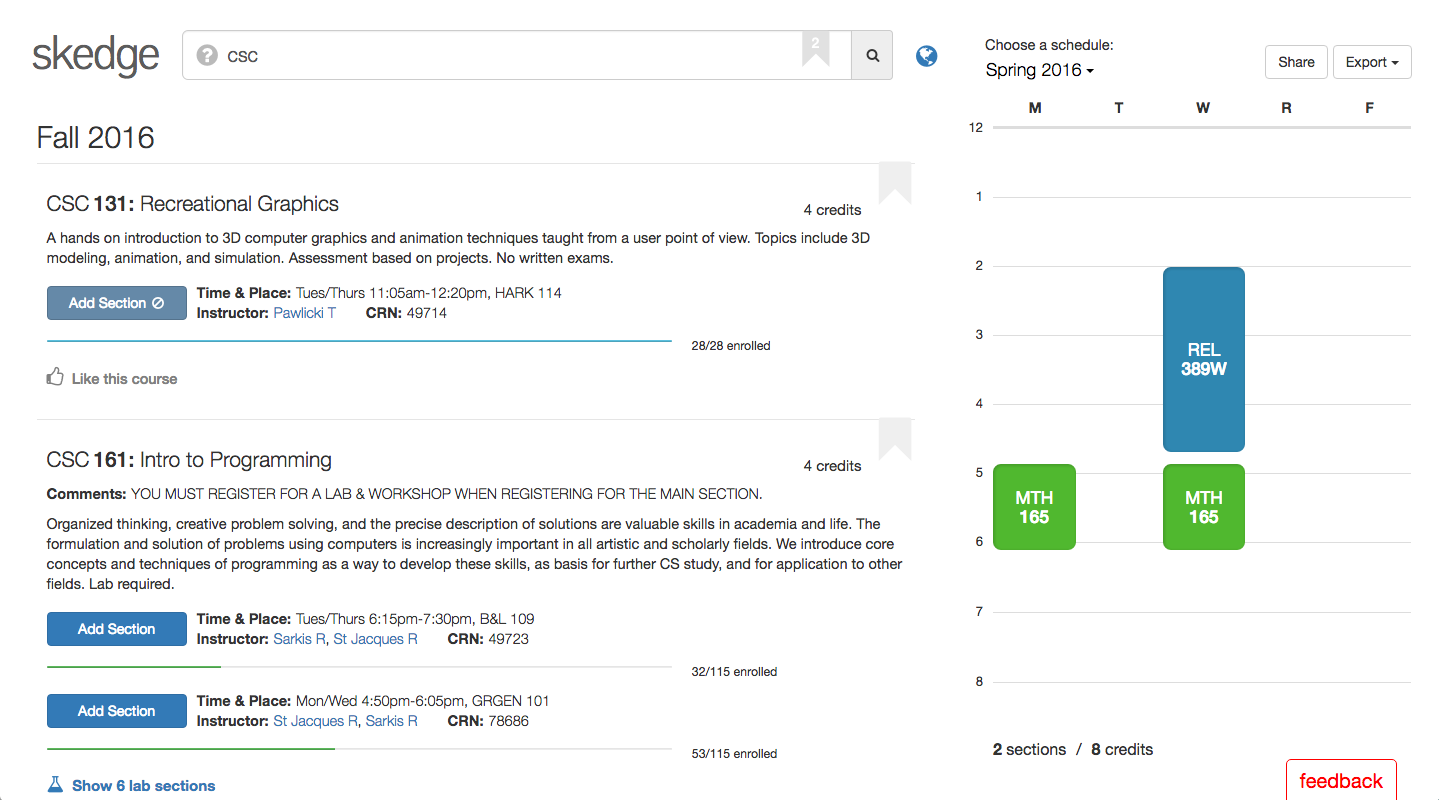
\includegraphics[width=1.00\textwidth]{images/skedge/index}
    }
    \caption[Skedge with the search query {\tt csc}]{Skedge with the search query {\tt csc} and the user's current schedule on the right}
    \label{fig:sk-index}
\end{figure}
\clearpage


\chapter{Design as a reaction to CDCS}

Improvements were made by USING CDCS, (bottom-up, not top-down)!

%%%

\section{Modernity}

CDCS is an old system.

\subsection{GET requests vs. AJAX}

- Can use back button
- Can send a link to a course or search

\subsection{Built-in scheduler vs. browser extension}

- Better UX
- Data is centralized

\subsection{Mobile}

- Important nowadays
- Mobile traffic stat or smth

\subsection{Public API}

- Important nowadays, extends student possibility
- JSON
- Brief demo of API

%%%

\section{Usability}

\subsection{Data quality}

- Courses don't shout
- Typos in comments
- 12-hour time

\subsection{Section display}

- Grouped course sections
- Embedded labs (A/B too), workshops, \& recitations

\subsection{Course reference}

- Clickable/hoverable course links, professor searches

\subsection{Multiple schedule support}

- Old CDCS+betterCDCS system can't keep track of this, have conflicts when adding stuff

\subsection{Exporting to GCal, .ics, image}

- Mobile sync support
- Security: BetterCDCS export gcal is currently broken and sends netID in PLAINTEXT over http(!!!)

\subsection{Search}

Most important usability concern is finding courses.

%%%

\section{Search}

Use cases, natural language.

\subsection{Course selection criteria}

Narrowed it down to three criteria. Keep in mind that \emph{none} of the things listed below are supported by CDCS, and they are all supported by Skedge.

  \subsubsection{Requirements}

  - Finding crosslists
  - Clusters

  \subsubsection{Browsing}

  - ``New'' courses
  - ``Autofit'' search
  - Random
  - Sorts

  \subsubsection{Friends}

  - ``What are my friends taking?'' (``what are you taking this semester'' = probably most common smalltalk phrase uttered on campus)
  - ``What do my friends recommend?'' - ``have you taken this class, and if so, what did you think of it?''

\subsection{Natural language search}

%Figure

See figure.

  \subsubsection{Advantages}

  - 15 fields reduced to 1

  vs form entry:
  - Faster
  - More intuitive
  - More easily extendable

  \subsubsection{Disadvantages}

  Having to know the DSL, grammar ambiguities (can be solved with a `did you mean')

\subsection{Multipurpose}

Used by other links (instructors, course references) around the site

\subsection{Added features}

- CRN (!)
- Crosslist
- Class size

%%%

\section{Social}

\subsection{The issue}

  \subsubsection{Static image vs. live site}

  - Edits don’t update
  - Referencing courses

  \subsubsection{Finding common courses}

  - requires your friends to share their schedules on FB publicly and you to see their post
  - is schedule-first, not search-first
  - typically only occurs for the current semester

%figure

\subsection{Skedge Social}

% Walkthru

  \subsubsection{Friends' course enrollments}

  Mini-feed

  \subsubsection{Friends' course likes}

  \subsubsection{Likes \& enrollments embedded in results}

  \subsubsection{Personal schedule synchronization}

  \subsubsection{Privacy}

  \subsubsection{Notifications}

  %figs of the 2 types
\clearpage


\chapter{Technical overview}

\section{Back-end}

\section{Front-end}

\section{Analytics}
\clearpage


\chapter{Data analytics}

Hypotheses:

1. Skedge's differences from and additions to CDCS are usable and have real need

2. Skedge’s navigations-per-add and other metrics demonstrate effectiveness of the use cases
a) direct searching, and
b) course browsing

3. Skedge’s DSL is user-friendly; users learn more advanced search types over time by using it

\section{Usage}

\subsection{General}

Since November 3rd 2015 (137 days)
3,768 unique users
4,500 schedules
Average 90 sessions/day
Average 4.92 pages/session
Average 5:31 minutes/session
28\% of sessions are from new users

MOBILE RESULT

\subsection{Search}

% figs

  \subsubsection{Empty searches}

  Can learn from these
  Some funny ones

\subsection{Course blocks}

40\% of sessions have at least one block-click
Average of 4.94 block-clicks per session

\subsection{Social}

90 users have linked Skedge to Facebook
Since March 1st,
4,000+ visits (200 visits/day)
~60\% of visits to /social were returning visitors
90 overlays onto friends’ schedules
10 clicks to Facebook profiles :(
- get stats from the fb dashboard

\subsection{Conclusion}

Success! Considering skedge is OPTIONAL.
+ course blocks (obv usecase, can't click)
+ exports (not supported by thing)
+ mobile

\section{Navigations-per-add}

\subsection{Definitions}

A navigation is defined as
a search, or
a click on an instructor’s name, or
a click on a crosslisted or prerequisite course link

The navigations-per-{add, bookmark} measure is
the number of navigations a user took (within one session) until a course was {added, bookmarked}

\subsection{Trends}

%figs

\subsection{Breaking them apart}

  behavioral patterns
  Direct search for specific course
  Discovery, browsing, exploring

  \subsubsection{Direct searches}

  \subsubsection{Browse}

  % STAT: Find major of users, find how many non-major courses they found

\subsection{Conclusion}

%figs

Effective++

\section{Users' search types over time}

\subsection{Definitions}

Points for search by (omits number and dept.):

description
credits
crosslisted
CRN
instructor
title
year
term
‘random’
upper-level writing

“CSC” → 0
“MTH 165” → 0
“taught by hema” → 1   ✓    (2 searches) 
“random mur 1-2 credits” → 2   ✓    (1 search) 


\subsection{Trends}

% fig

First increase (60.5% of users)
Median: 2 searches
Average: 4.23 searches
(Starting at 1 counts as an increase value of 0)

Second increase (7.9% of users)
Median: 8 searches
Average: 17.52 searches

\subsection{Conclusion}

DSL++
\clearpage


\chapter{Looking forward}

\section{Features}

\section{Analytics}
\clearpage


\chapter{Conclusions}

\section{Proposal to the University}

\section{Acknowledgments}

\section{Resources}

\subsection*{Source code}

The source code for Skedge is available online under an open source license:\\
\url{https://github.com/RocHack/skedge}.

\subsection*{Live site}

\noindent The site can be found at: \url{http://skedgeur.com}.
\clearpage

\begin{thebibliography}{1}

	\bibitem{markov} Takis Konstantopoulos {\em Introductory lecture notes on
		Markov Chains and Random Walks.} Uppsala University,
		\\\url{http://www2.math.uu.se/~takis/L/McRw/mcrw.pdf}

\end{thebibliography}

\addcontentsline{toc}{chapter}{Bibliography}

\clearpage
\section*{Appendix}

\end{document}
